%-----------------------------------------------------------------------------
%
%               Template for sigplanconf LaTeX Class
%
% Name:         sigplanconf-template.tex
%
% Purpose:      A template for sigplanconf.cls, which is a LaTeX 2e class
%               file for SIGPLAN conference proceedings.
%
% Guide:        Refer to "Author's Guide to the ACM SIGPLAN Class,"
%               sigplanconf-guide.pdf
%
% Author:       Paul C. Anagnostopoulos
%               Windfall Software
%               978 371-2316
%               paul@windfall.com
%
% Created:      15 February 2005
%
%-----------------------------------------------------------------------------


\documentclass[preprint,nocopyrightspace]{sigplanconf}

% The following \documentclass options may be useful:

% preprint      Remove this option only once the paper is in final form.
% 10pt          To set in 10-point type instead of 9-point.
% 11pt          To set in 11-point type instead of 9-point.
% authoryear    To obtain author/year citation style instead of numeric.

\usepackage{amsmath}
\usepackage{latexsym}
\usepackage{listings}
\usepackage[usenames]{xcolor}
\usepackage{lstcoq}
\usepackage{tikz}
\usepackage{pgfplots}

\usetikzlibrary{calc,positioning,decorations.markings,backgrounds}

\newcommand{\greg}[1]{\textcolor{blue}{\textsc{GREG}: #1}}


\begin{document}

\special{papersize=8.5in,11in}
\setlength{\pdfpageheight}{\paperheight}
\setlength{\pdfpagewidth}{\paperwidth}

\conferenceinfo{CONF 'yy}{Month d--d, 20yy, City, ST, Country}
\copyrightyear{20yy}
\copyrightdata{978-1-nnnn-nnnn-n/yy/mm}
\doi{nnnnnnn.nnnnnnn}

% Uncomment one of the following two, if you are not going for the
% traditional copyright transfer agreement.

%\exclusivelicense                % ACM gets exclusive license to publish,
                                  % you retain copyright

%\permissiontopublish             % ACM gets nonexclusive license to publish
                                  % (paid open-access papers,
                                  % short abstracts)

\titlebanner{}        % These are ignored unless
\preprintfooter{}   % 'preprint' option specified.

\title{Formal Verification of Stability Properties of Cyber-physical Systems}
%% \subtitle{Subtitle Text, if any}

\authorinfo{}
           {}
           {}
\authorinfo{}
           {}
           {}

\maketitle


% \category{CR-number}{subcategory}{third-level}

% % general terms are not compulsory anymore,
% % you may leave them out
% \terms
% term1, term2

% \keywords
% keyword1, keyword2

% intro, overview of project, overview of control theory, sketch of proof,
% future work
\section{Introduction}          % 1 col

We increasingly rely on computers to interact with the physical world for us.
At the large end, software underlies the control systems of commercial aircraft and power plants, and at the small end it controls medical devices and hobbiest UAVs.
The failure of any of these systems can have severe consequences which are often measured in the loss of human lives.
Formal verification has proven a promising approach to achieving very strong guarantees in more classic areas of computer science.
In this work we present an overview of our experiences formalizing stability properties of hybrid systems using the Coq proof assistant.

%% As we grow increasingly reliant on software for control of critical infrastructure, so does our need for guarantees that such software is free of errors. Complete formal verification with a proof assistant is the best way to obtain extremely strong guarantees that software systems satisfy a specification; however this technique has only recently been extended to the domain of cyber-physical systems [cite: ROScoq, MEMOCODE]. % is this true? Maybe a bit more here?
% In this paper, we present an overview of and our experiences in formalizing and reasoning about the physical behavior of hybrid systems in Coq.

In particular, we describe and contrast two approaches for proving the stability of a controller for a linear, one-dimensional hybrid system, depicted in Figure~\ref{fig:system-visualization}.
This system essentially runs in a loop in which the controller directly sets the velocity $v$ of the system and then the position $x$ evolves according to the differential equation $\dot{x} = v$ for at most $\Delta$ time while $v$ remains constant.
The goal of the controller is to move the system to a desired position, which, without loss of generality,  we assume to be 0.
The controller is a P controller, so-named because it sets the velocity to a value proportional to the difference between the current position and the desired position.

\section{System Specification}
\label{sec:veridrone}

We build our development on top of the VeriDrone project~\cite{ricketts2015veridrone}, a formalization of cyber-physical systems in the Coq proof assistant.
VeriDrone expresses cyber-physical systems and their properties uniformly in a linear temporal logic.
System specification generally take the form of the following temporal logic formula:
\begin{coq}
Init /\ $\Box$ (Discr \/ World)
\end{coq}
The first conjunct \coqe{Init} is a predicate over the initial state of the system.
The second conjunct (\coqe{$\Box$(...)}) expresses the transitions of the system.
In particular, it specifies that all temporally adjacent states are related by either \coqe{Discr}, a discrete transition that is morally of type \coqe{State -> State -> Prop}, or \coqe{World}, a continuous transition of the physical world expressed with predicates over the state and the time-derivative of variables in the state.
For our system depicted in Figure~\ref{fig:system-visualization}, these two types of transitions can be specified with
\begin{coq}
Discr := v' = -x/$\Delta$ /\ T' = t /\ t' = t /\ x' = x

World :=
 Cont (fun d => d x = v /\ d v = 0 /\ d t = 1 /\ d T = 0 /\ t - T < $\Delta$)
\end{coq}

In addition to the variables \coqe{x} and \coqe{v}, we need two additional variables to fully specify our system: \coqe{t}, tracking the current time of the system, and \coqe{T}, a stopwatch that is reset every time the P controller runs.
In the definition of \coqe{Discr}, \coqe{v' = -x/$\Delta$} specifies the P controller, \coqe{T' = t} specifies the resetting of the stopwatch, and \coqe{t' = t /\ x' = x} specify that the continuous variables do not change during the discrete transition.
In the definition of \coqe{World}, \coqe{d x = v} specifies the differential equation $\dot{x} = v$, \coqe{d v = 0} specifies that the velocity remains constant during continuous transitions, \coqe{d t = 1} specifies that \coqe{t} tracks the current time, \coqe{d T = 0} specifies that the stopwatch remains constant during continuous transitions, and \coqe{t - T < $\Delta$} specifies that less than $\Delta$ time elapses between executions of the controller.

\begin{figure}

\greg{Draw a figure representing the system}

\greg{Label discrete and continuous transitions}

\greg{Label the axes}


\scalebox{0.6}{% Created by tikzDevice version 0.8.1 on 2015-10-23 21:59:07
% !TEX encoding = UTF-8 Unicode
\documentclass[10pt]{article}
\usepackage{tikz}

\usepackage[active,tightpage,psfixbb]{preview}

\PreviewEnvironment{pgfpicture}

\setlength\PreviewBorder{0pt}
\begin{document}

\begin{tikzpicture}[x=1pt,y=1pt]
\definecolor{fillColor}{RGB}{255,255,255}
\path[use as bounding box,fill=fillColor,fill opacity=0.00] (0,0) rectangle (361.35,361.35);
\begin{scope}
\path[clip] ( 24.00, 48.00) rectangle (349.35,349.35);
\definecolor{drawColor}{RGB}{255,0,0}

\path[draw=drawColor,line width= 0.4pt,line join=round,line cap=round] ( 24.00,349.35) --
	( 35.22,310.52) --
	( 46.44,276.70) --
	( 57.66,247.23) --
	( 68.88,221.56) --
	( 80.09,199.20) --
	( 91.31,179.72) --
	(102.53,162.75) --
	(113.75,147.97) --
	(124.97,135.09) --
	(136.19,123.87) --
	(147.41,114.09) --
	(158.63,105.58) --
	(169.85, 98.16) --
	(181.07, 91.70) --
	(192.28, 86.07) --
	(203.50, 81.16) --
	(214.72, 76.89) --
	(225.94, 73.17) --
	(237.16, 69.92) --
	(248.38, 67.10) --
	(259.60, 64.64) --
	(270.82, 62.49) --
	(282.04, 60.63) --
	(293.26, 59.00) --
	(304.47, 57.58) --
	(315.69, 56.35) --
	(326.91, 55.27) --
	(338.13, 54.34) --
	(349.35, 53.52);
\end{scope}
\begin{scope}
\path[clip] (  0.00,  0.00) rectangle (361.35,361.35);
\definecolor{drawColor}{RGB}{0,0,0}

\path[draw=drawColor,line width= 0.4pt,line join=round,line cap=round] ( 24.00, 48.00) -- (349.35, 48.00);

\path[draw=drawColor,line width= 0.4pt,line join=round,line cap=round] ( 24.00, 48.00) -- ( 24.00, 42.00);

\path[draw=drawColor,line width= 0.4pt,line join=round,line cap=round] (105.34, 48.00) -- (105.34, 42.00);

\path[draw=drawColor,line width= 0.4pt,line join=round,line cap=round] (186.67, 48.00) -- (186.67, 42.00);

\path[draw=drawColor,line width= 0.4pt,line join=round,line cap=round] (268.01, 48.00) -- (268.01, 42.00);

\path[draw=drawColor,line width= 0.4pt,line join=round,line cap=round] (349.35, 48.00) -- (349.35, 42.00);

\node[text=drawColor,anchor=base,inner sep=0pt, outer sep=0pt, scale=  1.00] at ( 24.00, 26.40) {0};

\node[text=drawColor,anchor=base,inner sep=0pt, outer sep=0pt, scale=  1.00] at (105.34, 26.40) {1};

\node[text=drawColor,anchor=base,inner sep=0pt, outer sep=0pt, scale=  1.00] at (186.67, 26.40) {2};

\node[text=drawColor,anchor=base,inner sep=0pt, outer sep=0pt, scale=  1.00] at (268.01, 26.40) {3};

\node[text=drawColor,anchor=base,inner sep=0pt, outer sep=0pt, scale=  1.00] at (349.35, 26.40) {4};

\path[draw=drawColor,line width= 0.4pt,line join=round,line cap=round] ( 24.00,349.35) --
	( 24.00, 48.00) --
	(349.35, 48.00);
\end{scope}
\begin{scope}
\path[clip] (  0.00,  0.00) rectangle (361.35,361.35);
\definecolor{drawColor}{RGB}{0,0,0}

\node[text=drawColor,anchor=base,inner sep=0pt, outer sep=0pt, scale=  1.00] at (186.67,  2.40) {time};
\end{scope}
\begin{scope}
\path[clip] ( 24.00, 48.00) rectangle (349.35,349.35);
\definecolor{drawColor}{RGB}{0,0,0}

\node[text=drawColor,anchor=base west,inner sep=0pt, outer sep=0pt, scale=  1.30] at ( 76.81,223.35) {\itshape x};

\node[text=drawColor,anchor=base west,inner sep=0pt, outer sep=0pt, scale=  1.30] at ( 86.92,223.35) {=};

\node[text=drawColor,anchor=base west,inner sep=0pt, outer sep=0pt, scale=  1.30] at (100.27,223.35) {-};

\node[text=drawColor,anchor=base west,inner sep=0pt, outer sep=0pt, scale=  1.30] at (106.54,223.35) {a};

\node[text=drawColor,anchor=base west,inner sep=0pt, outer sep=0pt, scale=  1.30] at (113.04,223.35) {\itshape e};

\node[text=drawColor,anchor=base west,inner sep=0pt, outer sep=0pt, scale=  0.91] at (119.86,228.67) {\itshape t};

\node[text=drawColor,anchor=base west,inner sep=0pt, outer sep=0pt, scale=  0.91] at (123.72,228.67) {-};

\node[text=drawColor,anchor=base west,inner sep=0pt, outer sep=0pt, scale=  0.91] at (126.75,228.67) {\itshape t};

\node[text=drawColor,anchor=base west,inner sep=0pt, outer sep=0pt, scale=  0.65] at (130.61,227.30) {0};
\end{scope}
\begin{scope}
\path[clip] (  0.00,  0.00) rectangle (361.35,361.35);
\definecolor{drawColor}{RGB}{0,0,0}

\path[draw=drawColor,line width= 0.4pt,line join=round,line cap=round] ( 24.00, 48.00) -- (349.35, 48.00);

\path[draw=drawColor,line width= 0.4pt,line join=round,line cap=round] ( 24.00, 48.00) -- ( 24.00, 48.00);

\path[draw=drawColor,line width= 0.4pt,line join=round,line cap=round] (349.35, 48.00) -- (349.35, 48.00);
\end{scope}
\begin{scope}
\path[clip] ( 24.00, 48.00) rectangle (349.35,349.35);
\definecolor{drawColor}{RGB}{0,0,0}

\path[draw=drawColor,line width= 0.4pt,line join=round,line cap=round] ( 32.13,252.92) --
	( 80.94,126.35) --
	(129.74,108.27) --
	(146.01, 90.19) --
	(251.74, 60.05) --
	(316.81, 54.03);

\node[text=drawColor,anchor=base west,inner sep=0pt, outer sep=0pt, scale=  1.12] at ( 24.96,256.13) {(};

\node[text=drawColor,anchor=base west,inner sep=0pt, outer sep=0pt, scale=  0.90] at ( 29.33,256.13) {\itshape t};

\node[text=drawColor,anchor=base west,inner sep=0pt, outer sep=0pt, scale=  0.63] at ( 33.15,254.78) {0};

\node[text=drawColor,anchor=base west,inner sep=0pt, outer sep=0pt, scale=  0.90] at ( 36.30,256.13) {,};

\node[text=drawColor,anchor=base west,inner sep=0pt, outer sep=0pt, scale=  0.90] at ( 38.80,256.13) { };

\node[text=drawColor,anchor=base west,inner sep=0pt, outer sep=0pt, scale=  0.90] at ( 43.30,256.13) {\itshape x};

\node[text=drawColor,anchor=base west,inner sep=0pt, outer sep=0pt, scale=  0.63] at ( 48.05,254.78) {0};

\node[text=drawColor,anchor=base west,inner sep=0pt, outer sep=0pt, scale=  1.12] at ( 51.20,256.13) {)};

\path[draw=drawColor,line width= 0.4pt,line join=round,line cap=round] ( 78.69,124.10) -- ( 83.19,128.60);

\path[draw=drawColor,line width= 0.4pt,line join=round,line cap=round] ( 78.69,128.60) -- ( 83.19,124.10);

\path[draw=drawColor,line width= 0.4pt,line join=round,line cap=round] (127.49,106.02) -- (131.99,110.52);

\path[draw=drawColor,line width= 0.4pt,line join=round,line cap=round] (127.49,110.52) -- (131.99,106.02);

\path[draw=drawColor,line width= 0.4pt,line join=round,line cap=round] (143.76, 87.94) -- (148.26, 92.44);

\path[draw=drawColor,line width= 0.4pt,line join=round,line cap=round] (143.76, 92.44) -- (148.26, 87.94);

\path[draw=drawColor,line width= 0.4pt,line join=round,line cap=round] (249.49, 57.80) -- (253.99, 62.30);

\path[draw=drawColor,line width= 0.4pt,line join=round,line cap=round] (249.49, 62.30) -- (253.99, 57.80);

\path[draw=drawColor,line width= 0.4pt,line join=round,line cap=round] (314.56, 51.78) -- (319.06, 56.28);

\path[draw=drawColor,line width= 0.4pt,line join=round,line cap=round] (314.56, 56.28) -- (319.06, 51.78);

\path[draw=drawColor,line width= 0.4pt,line join=round,line cap=round] ( 29.88,250.67) -- ( 34.38,255.17);

\path[draw=drawColor,line width= 0.4pt,line join=round,line cap=round] ( 29.88,255.17) -- ( 34.38,250.67);
\end{scope}
\end{tikzpicture}

\end{document}
}

\caption{Visualization of a P-controller}
\label{fig:system-visualization}
\end{figure}


%% The Veridrone project aims to build cyber-physical systems that adhere to various safety policies, by proving that various formal specifications are obeyed in Coq. Our work is implemented in the domain of hobbyist unmanned aerial vehicles (drones), described in .... We have constructed shims for bounding velocity and height, and shown how to compose them in [cite]. In this paper, we present our experiences in formalizing and reasoning about stability properties of the quadcopter.

%In order to avoid formalizing the entirety of the existing control software, we simply guard the feedback loop by inserting verified shims between the existing software and the actuators.



% start with the proof goal then introduce stability, or stability -> different proofs of stability?

\section{Stability}

In this work we use the Veridrone system to reason about ``stability'' in the control theory sense.
Stability is a classic property from control theory that captures a temporal notion of boundedness in terms of distance from a goal point.
There are three levels of stability which are shown graphically in Figure~\ref{fig:stability}:


\begin{figure}[!h]
  \centering
  \resizebox{\linewidth}{0.8\linewidth}{% Created by tikzDevice version 0.8.1 on 2015-10-23 16:26:30
% !TEX encoding = UTF-8 Unicode
\begin{tikzpicture}[x=1pt,y=1pt]
\definecolor{fillColor}{RGB}{255,255,255}
\path[use as bounding box,fill=fillColor,fill opacity=0.00] (0,0) rectangle (361.35,361.35);
\begin{scope}
\path[clip] (  0.00,  0.00) rectangle (361.35,361.35);
\definecolor{drawColor}{RGB}{0,0,0}

\path[draw=drawColor,line width= 0.4pt,line join=round,line cap=round] ( 24.00, 45.73) -- ( 24.00,315.61);

\path[draw=drawColor,line width= 0.4pt,line join=round,line cap=round] ( 24.00, 45.73) -- ( 18.00, 45.73);

\path[draw=drawColor,line width= 0.4pt,line join=round,line cap=round] ( 24.00,113.20) -- ( 18.00,113.20);

\path[draw=drawColor,line width= 0.4pt,line join=round,line cap=round] ( 24.00,180.67) -- ( 18.00,180.67);

\path[draw=drawColor,line width= 0.4pt,line join=round,line cap=round] ( 24.00,248.14) -- ( 18.00,248.14);

\path[draw=drawColor,line width= 0.4pt,line join=round,line cap=round] ( 24.00,315.61) -- ( 18.00,315.61);

\node[text=drawColor,rotate= 90.00,anchor=base,inner sep=0pt, outer sep=0pt, scale=  1.00] at (  9.60, 45.73) {-4};

\node[text=drawColor,rotate= 90.00,anchor=base,inner sep=0pt, outer sep=0pt, scale=  1.00] at (  9.60,113.20) {-2};

\node[text=drawColor,rotate= 90.00,anchor=base,inner sep=0pt, outer sep=0pt, scale=  1.00] at (  9.60,180.67) {0};

\node[text=drawColor,rotate= 90.00,anchor=base,inner sep=0pt, outer sep=0pt, scale=  1.00] at (  9.60,248.14) {2};

\node[text=drawColor,rotate= 90.00,anchor=base,inner sep=0pt, outer sep=0pt, scale=  1.00] at (  9.60,315.61) {4};
\end{scope}
\begin{scope}
\path[clip] (  0.00,  0.00) rectangle (361.35,361.35);
\definecolor{drawColor}{RGB}{255,0,0}

\path[draw=drawColor,line width= 0.4pt,line join=round,line cap=round] ( 24.00,281.88) -- (349.35,281.88);

\path[draw=drawColor,line width= 0.4pt,line join=round,line cap=round] ( 24.00, 79.47) -- (349.35, 79.47);
\definecolor{drawColor}{RGB}{0,0,0}

\path[draw=drawColor,line width= 0.4pt,line join=round,line cap=round] ( 24.00,214.41) --
	( 27.41,175.77) --
	( 48.28,186.02) --
	( 81.88,110.86) --
	( 97.64,267.47) --
	(113.63,174.11) --
	(117.59,221.17) --
	(125.93,136.39) --
	(184.97,274.09) --
	(336.47, 88.30) --
	(346.34,121.38);

\path[draw=drawColor,line width= 0.4pt,line join=round,line cap=round] (115.34,218.92) -- (119.84,223.42);

\path[draw=drawColor,line width= 0.4pt,line join=round,line cap=round] (115.34,223.42) -- (119.84,218.92);

\path[draw=drawColor,line width= 0.4pt,line join=round,line cap=round] ( 79.63,108.61) -- ( 84.13,113.11);

\path[draw=drawColor,line width= 0.4pt,line join=round,line cap=round] ( 79.63,113.11) -- ( 84.13,108.61);

\path[draw=drawColor,line width= 0.4pt,line join=round,line cap=round] (123.68,134.14) -- (128.18,138.64);

\path[draw=drawColor,line width= 0.4pt,line join=round,line cap=round] (123.68,138.64) -- (128.18,134.14);

\path[draw=drawColor,line width= 0.4pt,line join=round,line cap=round] ( 25.16,173.52) -- ( 29.66,178.02);

\path[draw=drawColor,line width= 0.4pt,line join=round,line cap=round] ( 25.16,178.02) -- ( 29.66,173.52);

\path[draw=drawColor,line width= 0.4pt,line join=round,line cap=round] (182.72,271.84) -- (187.22,276.34);

\path[draw=drawColor,line width= 0.4pt,line join=round,line cap=round] (182.72,276.34) -- (187.22,271.84);

\path[draw=drawColor,line width= 0.4pt,line join=round,line cap=round] (344.09,119.13) -- (348.59,123.63);

\path[draw=drawColor,line width= 0.4pt,line join=round,line cap=round] (344.09,123.63) -- (348.59,119.13);

\path[draw=drawColor,line width= 0.4pt,line join=round,line cap=round] (334.22, 86.05) -- (338.72, 90.55);

\path[draw=drawColor,line width= 0.4pt,line join=round,line cap=round] (334.22, 90.55) -- (338.72, 86.05);

\path[draw=drawColor,line width= 0.4pt,line join=round,line cap=round] ( 95.39,265.22) -- ( 99.89,269.72);

\path[draw=drawColor,line width= 0.4pt,line join=round,line cap=round] ( 95.39,269.72) -- ( 99.89,265.22);

\path[draw=drawColor,line width= 0.4pt,line join=round,line cap=round] (111.38,171.86) -- (115.88,176.36);

\path[draw=drawColor,line width= 0.4pt,line join=round,line cap=round] (111.38,176.36) -- (115.88,171.86);

\path[draw=drawColor,line width= 0.4pt,line join=round,line cap=round] ( 46.03,183.77) -- ( 50.53,188.27);

\path[draw=drawColor,line width= 0.4pt,line join=round,line cap=round] ( 46.03,188.27) -- ( 50.53,183.77);

\path[draw=drawColor,line width= 0.4pt,line join=round,line cap=round] ( 21.75,212.16) -- ( 26.25,216.66);

\path[draw=drawColor,line width= 0.4pt,line join=round,line cap=round] ( 21.75,216.66) -- ( 26.25,212.16);
\end{scope}
\end{tikzpicture}
}

  (a) Lyapunov stability

  \resizebox{\linewidth}{0.8\linewidth}{% Created by tikzDevice version 0.8.1 on 2015-10-22 05:37:53
% !TEX encoding = UTF-8 Unicode
\begin{tikzpicture}[x=1pt,y=1pt]
\definecolor{fillColor}{RGB}{255,255,255}
\path[use as bounding box,fill=fillColor,fill opacity=0.00] (0,0) rectangle (361.35,361.35);
\begin{scope}
\path[clip] ( 49.20, 61.20) rectangle (336.15,312.15);
\definecolor{drawColor}{RGB}{0,0,0}

\path[draw=drawColor,line width= 0.4pt,line join=round,line cap=round] ( 59.83,302.86) --
	( 68.99,287.89) --
	( 78.15,274.85) --
	( 87.31,263.49) --
	( 96.48,253.59) --
	(105.64,244.97) --
	(114.80,237.46) --
	(123.96,230.91) --
	(133.12,225.22) --
	(142.28,220.25) --
	(151.45,215.92) --
	(160.61,212.16) --
	(169.77,208.87) --
	(178.93,206.01) --
	(188.09,203.52) --
	(197.26,201.35) --
	(206.42,199.46) --
	(215.58,197.81) --
	(224.74,196.38) --
	(233.90,195.13) --
	(243.07,194.04) --
	(252.23,193.09) --
	(261.39,192.26) --
	(270.55,191.54) --
	(279.71,190.92) --
	(288.87,190.37) --
	(298.04,189.89) --
	(307.20,189.48) --
	(316.36,189.12) --
	(325.52,188.80);
\end{scope}
\begin{scope}
\path[clip] (  0.00,  0.00) rectangle (361.35,361.35);
\definecolor{drawColor}{RGB}{0,0,0}

\path[draw=drawColor,line width= 0.4pt,line join=round,line cap=round] ( 59.83,186.67) -- (325.52,186.67);

\path[draw=drawColor,line width= 0.4pt,line join=round,line cap=round] ( 59.83,186.67) -- ( 59.83,186.67);

\path[draw=drawColor,line width= 0.4pt,line join=round,line cap=round] (325.52,186.67) -- (325.52,186.67);

\path[draw=drawColor,line width= 0.4pt,line join=round,line cap=round] ( 59.83, 93.73) -- ( 59.83,279.62);

\path[draw=drawColor,line width= 0.4pt,line join=round,line cap=round] ( 59.83, 93.73) -- ( 59.83, 93.73);

\path[draw=drawColor,line width= 0.4pt,line join=round,line cap=round] ( 59.83,186.67) -- ( 59.83,186.67);

\path[draw=drawColor,line width= 0.4pt,line join=round,line cap=round] ( 59.83,279.62) -- ( 59.83,279.62);

\node[text=drawColor,rotate= 90.00,anchor=base,inner sep=0pt, outer sep=0pt, scale=  1.00] at ( 45.43,186.67) {0};
\end{scope}
\begin{scope}
\path[clip] ( 49.20, 61.20) rectangle (336.15,312.15);
\definecolor{drawColor}{RGB}{0,0,0}

\path[draw=drawColor,line width= 0.4pt,line join=round,line cap=round] ( 59.83, 70.49) --
	( 62.48, 75.05) --
	( 65.14, 79.43) --
	( 67.80, 83.63) --
	( 70.46, 87.67) --
	( 73.11, 91.55) --
	( 75.77, 95.28) --
	( 78.43, 98.87) --
	( 81.08,102.31) --
	( 83.74,105.62) --
	( 86.40,108.80) --
	( 89.05,111.85) --
	( 91.71,114.78) --
	( 94.37,117.60) --
	( 97.02,120.31) --
	( 99.68,122.91) --
	(102.34,125.41) --
	(105.00,127.82) --
	(107.65,130.12) --
	(110.31,132.34) --
	(112.97,134.47) --
	(115.62,136.52) --
	(118.28,138.49) --
	(120.94,140.37) --
	(123.59,142.19) --
	(126.25,143.93) --
	(128.91,145.61) --
	(131.57,147.22) --
	(134.22,148.77) --
	(136.88,150.25) --
	(139.54,151.68) --
	(142.19,153.05) --
	(144.85,154.37) --
	(147.51,155.64) --
	(150.16,156.86) --
	(152.82,158.03) --
	(155.48,159.15) --
	(158.13,160.23) --
	(160.79,161.26) --
	(163.45,162.26) --
	(166.11,163.22) --
	(168.76,164.14) --
	(171.42,165.02) --
	(174.08,165.87) --
	(176.73,166.69) --
	(179.39,167.47) --
	(182.05,168.22) --
	(184.70,168.95) --
	(187.36,169.64) --
	(190.02,170.31) --
	(192.67,170.95) --
	(195.33,171.57) --
	(197.99,172.16) --
	(200.65,172.73) --
	(203.30,173.28) --
	(205.96,173.80) --
	(208.62,174.31) --
	(211.27,174.79) --
	(213.93,175.26) --
	(216.59,175.71) --
	(219.24,176.14) --
	(221.90,176.55) --
	(224.56,176.95) --
	(227.22,177.33) --
	(229.87,177.69) --
	(232.53,178.05) --
	(235.19,178.38) --
	(237.84,178.71) --
	(240.50,179.02) --
	(243.16,179.32) --
	(245.81,179.61) --
	(248.47,179.89) --
	(251.13,180.15) --
	(253.78,180.41) --
	(256.44,180.65) --
	(259.10,180.89) --
	(261.76,181.12) --
	(264.41,181.34) --
	(267.07,181.54) --
	(269.73,181.75) --
	(272.38,181.94) --
	(275.04,182.12) --
	(277.70,182.30) --
	(280.35,182.47) --
	(283.01,182.64) --
	(285.67,182.80) --
	(288.32,182.95) --
	(290.98,183.10) --
	(293.64,183.24) --
	(296.30,183.37) --
	(298.95,183.50) --
	(301.61,183.62) --
	(304.27,183.74) --
	(306.92,183.86) --
	(309.58,183.97) --
	(312.24,184.08) --
	(314.89,184.18) --
	(317.55,184.28) --
	(320.21,184.37) --
	(322.87,184.46) --
	(325.52,184.55);

\path[draw=drawColor,line width= 0.4pt,line join=round,line cap=round] ( 66.47,244.77) --
	( 98.88,223.89) --
	(143.58,172.69) --
	(214.49,195.35) --
	(292.96,186.04);

\path[draw=drawColor,line width= 0.4pt,line join=round,line cap=round] (141.33,170.44) -- (145.83,174.94);

\path[draw=drawColor,line width= 0.4pt,line join=round,line cap=round] (141.33,174.94) -- (145.83,170.44);

\path[draw=drawColor,line width= 0.4pt,line join=round,line cap=round] ( 96.63,221.64) -- (101.13,226.14);

\path[draw=drawColor,line width= 0.4pt,line join=round,line cap=round] ( 96.63,226.14) -- (101.13,221.64);

\path[draw=drawColor,line width= 0.4pt,line join=round,line cap=round] (290.71,183.79) -- (295.21,188.29);

\path[draw=drawColor,line width= 0.4pt,line join=round,line cap=round] (290.71,188.29) -- (295.21,183.79);

\path[draw=drawColor,line width= 0.4pt,line join=round,line cap=round] (212.24,193.10) -- (216.74,197.60);

\path[draw=drawColor,line width= 0.4pt,line join=round,line cap=round] (212.24,197.60) -- (216.74,193.10);

\path[draw=drawColor,line width= 0.4pt,line join=round,line cap=round] ( 64.22,242.52) -- ( 68.72,247.02);

\path[draw=drawColor,line width= 0.4pt,line join=round,line cap=round] ( 64.22,247.02) -- ( 68.72,242.52);
\end{scope}
\end{tikzpicture}
}

  (a) Exponential stability

  \caption{Visualzation for (a) Lyapunov and (b) exponential stability.}
  \label{fig:stability}
\end{figure}


\begin{enumerate}
\item \textbf{Lyapunov stability} states that if the system starts within $\beta > 0$ from the goal, then it will stay within $\alpha$ of the goal point for all time.
In our temporal logic, \coqe{x} is Lyapunov stable if
\begin{coq}
Definition LyapunovStable ($x$ : Term) : Formula :=
  Forall $\alpha$ : R, $\alpha$ > 0 -> (* boundary *)
    Exists $\beta$ : R, $\beta$ > 0 /\ (* start *)
      (|$x$| < $\beta$) -> $\Box$(|$x$| < $\alpha$).
\end{coq}
Note that the universal quantification of the boundary implies that if the system starts arbitrarily close, then it will remain arbitrarily close.
However, the definition does not imply that the system converges.
For example, the system that stays a constant distance from the goal is Lyapunov stable.

%%\item \textbf{Asymptotic stability} states that the distance from the goal is bounded by a decreasing function of time.
%% Formally, this is expressed by the following definition:

\item \textbf{Exponential stability} is a refinement of stability that guarantees that the system converges to the goal exponentially fast.
The formal definition is the following:
\begin{coq}
Definition ExpStable (x : Term) : Formula :=
  Exists $\alpha$ : R, $\alpha$ > 0 /\ Exists $\beta$ : R, $\beta$ > 0 /\
  Exists $x_0$: R, $x$ = $x_0$ /\ Exists $t_0$ : R, $t_0$ = $\tau$ /\
     $\Box$(|$x$| $\leq$ ($\alpha$ * |$x_0$| * e^{-$\beta$ * ($\tau$ - $t_0$)}).
\end{coq}
The first line existentially quantifies both $\alpha$ and $\beta$, and the second line captures the initial configuration (time in $t_0$ and the value of $x$ in $x_0$).
In this definition $\tau$ is the global time which increases monotonically, i.e. we must prove that our system is confined by a single exponential regardless of the number of discrete and continuous transitions it takes.

\end{enumerate}

%% These definitions form a heirarchy of stability.
%% All asymptotically stable systems are Lyapunov stable, and all exponentially stable systems are asymptotically stable.

\section{Proving Stability Directly}
\label{sec:graphical}

We began by proving that our system is Lyapunov stable using basic temporal logic induction.
While cumbersome due to the heavy use of arithmetic, the proof is quite similar to those performed when verifying safety properties of monitors in the VeriDrone~\cite{ricketts2015veridrone} work.
The proof proceeds in two steps.
First, we assume that $x$ is positive and we prove that the value of $x$ does not increase over time and further, never becomes negative.
Then, by symmetry we can reuse this proof to justify the lower-bound by ``flipping the proof'' over the time axis.

\paragraph{Exponential Stability}
We are currently in the process of proving the same controller exponentially stabile.
The proof is more subtle because we need to justify that the rate at which the sytem approaches the goal is greater than the rate at which the exponential function approaches the goal, which itself is a function of the time since the start.
However, the controller is time-invariant, i.e. its output does not depend directly on time.
This requires us to relate the slope of the exponential directly to the current value of $x$.

Figure~\ref{fig:graphical-proof} provides a graphical sketch of the reasoning.
As with the Lyapunov stability proof, we can just consider positive values of $x$.
We will pick $\alpha = 1$ and $\beta = \frac{1}{\beta}$.
The choice of $\beta$ here is essential for this particular controller.
In particular, note that the velocity chosen by the controller $-\frac{x}{\delta}$ is exactly the slope of the exponential \emph{where it crosses the horizontal line through $x$}.
Therefore, the tragectory of the system is parallel to the tangent line.
Since the exponential is concave up it is always greater than its tangent line (a fact we proved in Coq).
Therefore, by transitivity our location is always below the exponential during continuous transitions.
We have completed this proof in Coq.

While this appears to be the crux of the proof, it is not complete.
In particular, it only handles the continuous transition.
In order to extend the proof to the hybrid system, we must extend the proof to address the discrete transitions which has been more difficult than we anticipated.
%% The central difficulty, as with many verification efforts, lies in the inductive hypothesis.
%% While a similar proof methodology to the Lyapunov stability proof should work, we have been focused on a separation of parameters.




%% Since this domain is naturally a visual one, our first approach to proving stability is inspired by informal graphical proofs of Lyapunov stability and exponential stability of the controller described in Section~\ref{sec:veridrone}.
%% Here, we focus on the proof of exponential stability.
%% The graphical proof of exponential stability is depicted in Figure~\ref{fig:graphical-proof}.

\begin{figure}
\centering
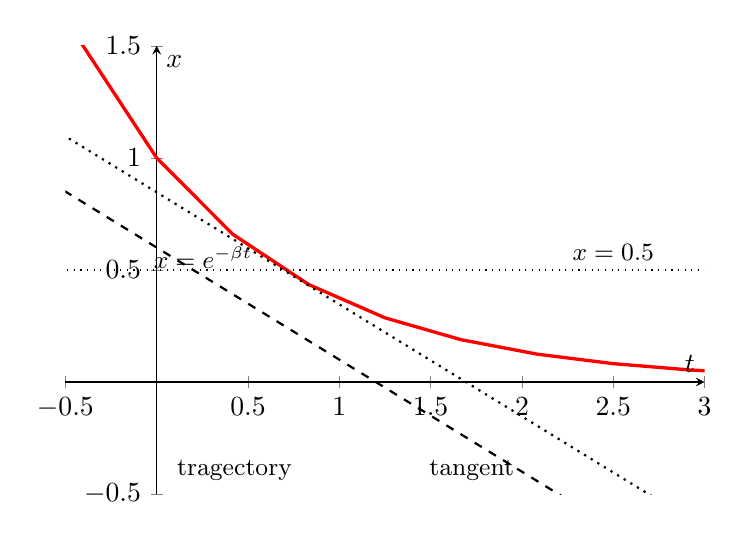
\begin{tikzpicture}
\begin{axis}[height=0.6\linewidth,width=0.8\linewidth,
          xmin=-0.5,xmax=3,ymax=1.5,ymin=-0.5,
          axis lines=middle,
          xlabel=$t$,
          ylabel=$x$]
\addplot[red,very thick]  {pow(e,-1*x)} ; %% node[above]{$x=e^{-\beta t}$};
\addplot[black,dotted,thick] {-0.5 * (x + ln(0.5)) + 0.5} ; %% node[pos=0.75,right]{\tiny$x=\ln 0.5 + 0.5$};
\addplot[black,dashed,thick] {-0.5 * (x - 0.2) + 0.5} ; %% node[below]{$x=\ln 0.5 + 0.5$};
\addplot[black,dotted] {0.5} node[above,pos=0.75] {\small $x=0.5$};
\end{axis}
\node[anchor=west] at (1,3) {\small $x=e^{-\beta t}$} ;
\node[anchor=west] at (4.5,0.3) {\small tangent} ;
\node[anchor=east] at (3,0.3) {\small tragectory} ;
\end{tikzpicture}

\caption{Graphical ``proof'' of exponential stability.}
\label{fig:graphical-proof}
\end{figure}

%% An important safety property we would like guarantees about is that of \emph{stability}. Given deceleration $d$, will our quadcopter eventually come to a stop? Or, given initial velocity $v$, will the quadcopter reach a target coordinate $c$? How quickly can it reach the target?

%% In control theory, stability formalizes these properties about a given system. Formally, it aims to show whether a set of differential equations will converge to a fixed point over time given some initial conditions. The challenge with applying the standard techniques from control theory to the domain of hybrid systems is in reasoning about both discrete and continuous aspects

% Canonically, there are three tiers of stability ---



% We have proven Lyapunov and Exponential stability for our height controller, which bounds the deceleration behavior of the quadcopter.

% something about TLA, the Sys abstraction and differential induction

% 1. Lyapunov stability

% 2. Exponential stability

% Exponential stability states that the continuous dynamics of the system will force the quadcopter to land exponentially fast --- that is,

% starting at an initial state

%% In order to formalize this graphical proof in Coq, we ...

%% In the time interval between runs of the discrete controller, $t_0\leq t \leq t_0+\Delta$, the height of the system will decrease exponentially fast over multiple continuous transitions of the system, with its upper bound given by the function
%%  \[E(t)=x_0e^{-b(t-t_0)}\]
%% but this leaves us with the unpleasant work of having to reason over fractionals. In order to simplify our proofs, we instead assert a stronger property --- that the height is bounded by the tangent to $E$ at $t_0$, selected at the start of the continuous transitions:
%% \[T(t) = E'(t_0)(t-t_0)+x_0 = -bx_0(t-t_0)+x_0\]
%% which we can then compose into a proof of exponential stability by showing that
%% \[
%%   \frac
%%   {\begin{aligned}
%%       & \vdash \emph{Init} \land \Box \emph{World} \rightarrow \Box \emph{Safe} \\
%%       & \vdash \Box (T\leq E)
%%     \end{aligned}}
%%   {\vdash \emph{Init} \land \Box \emph{World} \rightarrow \Box \emph{ExpSafe}}
%% \]

% Exponential stability of height over time: $E(t)=x_0e^{-b(t-t_0)}$
% tangent to Exp: \[T(t) = E'(t_0)(t-t_0)+x_0 = -bx_0(t-t_0)+x_0\]


% Should this be folded into the narrative about the two stability proofs?
% Or should this describe the interesting parts of the proofs while the above
% describes the math? .... what really do I put here?

\section{Stability Proofs using Lyapunov Functions}
\label{sec:lyapunov-functions}

In addition to the visually appealing approach described in Section~\ref{sec:graphical}, we have also begun exploring the potential of proving stability using a standard approach from control theory: Lyapunov functions.
Very roughly speaking, Lyapunov functions allow one to prove stability of a system using some notion of the energy of the system in which the energy is 0 at the equilibrium, positive elsewhere, and decreases over time.
More precisely, a Lyapunov function for a one-dimensional system with an equilibrium at 0 is a function $V : \mathcal{R} \rightarrow \mathcal{R}$ such that $V(0) = 0$, $V(x) > 0$ for $x \neq 0$, and satisfying some condition on the time-derivative $\dot{V(x)}$.

This condition on $\dot{V(x)}$ depends on the particular notion of stability one would like to prove.
For Lyapunov stability, asymptotic stability, and exponential stability, the conditions are $\dot{V(x)} \leq 0$, $\dot{V(x)} < 0$, and $\dot{V(x)} \leq \alpha V(x)$ for $\alpha < 0$, respectively.

For a purely continuous P controller, specified by the differential equation $\dot{x} = -x$, the function $V(x) = \frac{1}{2}x^2$ serves as a Lyapunov function satisfying all three conditions on the time-derivative and thus estabilishes all three notions of stability.
To see this, note that $\dot{V(x)} = x\dot{x} = -x^2$.
Unfortunately, for our hybrid P controller, the same computation gives us $\dot{V(x)} = x\dot{x} = x*v$.
However, we can prove that our P controller is a refinement of the system in which $\dot{x} = \frac{-x}{\Delta - (t - T)}$.
In other words, the velocity is proportional to the distance from the equilibrium and inversely proportional to the time remaining before the controller must run again.
Using this abstraction, it is possible to establish all three conditions on the time derivative of $V$ and hence all three notions of stability.
Thus far, we have only fully formalized in Coq the proof of Lyapunov stability of our P controller using a Lyapunov function.

\section {Experiences}

It is interesting to contrast the process of formalizing the graphically-inspired proofs with the proofs based on Lyapunov functions.
Though the graphically-inspired proofs appear to be simpler and more intuitive on paper, our initial experience suggests that they are more challenging to formalize due to a lack of abstraction of time.
Lyapunov functions provide such an abstraction and hence seem to provide an cleaner path to a fully formal proof.
However, the time-abstraction seems to break slightly when one uses Lyapunov functions for a hybrid system rather than a purely continuous system.
More investigation is necessary to determine how both of these approaches scale to more complex hybrid systems.

% \emph{Coq as a reasoning tool: } Following several unsuccessful attempts to extend the proof of Lyapunov stability for exponential stability, we discovered that contrary to the hierarchy of mathematical definitions, the context that the two proofs needed are different. Because of the weakness of Lyapunov stability, we were able to correctly formulate it assuming that the


% This uncovered an interesting property about the interactions between the discrete and continuous parts of hybrid systems --- that

%  Intuitively, Lyapunov stability is a property that holds true for \emph{all time}, while asymptotic and exponential stability converge, and can be thought of as a piecewise function that becomes constant after the stable point is reached. did not realize this

% forced us to reexamine our formalism
% ... pointed out gaps in our reasoning.


% \emph{Reasoning about real arithmetic, powers and floating point: }
% A significant challenge faced during our development of the proofs, especially the

\section{Future work}

Our initial work on stability has focused on a one-dimensional P (Proportional) controller. By extending the model to the full generality of a PID (Proportional-Integral-Derivative) controller, which will allow for the expression of more exciting behaviors such as oscillatory convergence to a goal, rather than limiting behavior to be monotonically increasing or decreasing towards the goal as it is in the current formulation.

Ideally, the construction of a verified PID controller would follow from a layered composition, allowing for the separate construction of the I and D controllers. It might prove helpful to reformulate our mathematics using the standard method of Lyapunov functions from control theory, which in principle would allow for the different types of stability to be expressed in a uniform way. In the context of hybrid systems, however, Lyapunov's method might need to be extended to incorporate the discrete component.


% Logical extensions to this work would be to show the convergence of the system in the remaining two dimensions, so as to guarantee that we can accurately reach any point in three dimensional space. To this end, . Further refinements on the


% Have to figure out how our formalism maps to PID controller theory
% ... PID (Proportional-Integral-Derivative) controllers.
% - Proportional gain
% - Integral - accelerates movement towards stable point. accounts for both positive and neg errors
% - Derivative -

% - use lyapunov functions - continuous, not hybrid. need a formalism for hybrid systems
% - higher order PI and PID controllers
% - composing controllers





% \appendix
% \section{Appendix Title}

% This is the text of the appendix, if you need one.

% \acks

% Acknowledgments, if needed.

% We recommend abbrvnat bibliography style.

\bibliographystyle{abbrvnat}

% The bibliography should be embedded for final submission.

\begin{thebibliography}{}
\softraggedright
% ROScoq: http://www.cs.cornell.edu/~aa755/ROSCoq/
% Stability defns: Murray et al, "A mathematical introduction to robotic manipulation, ch4"
% http://www.cds.caltech.edu/~murray/courses/cds101/fa02/caltech/mls93-lyap.pdf
\bibitem[Smith et~al.(2009)Smith, Jones]{smith02}
P. Q. Smith, and X. Y. Jones. ...reference text...

\end{thebibliography}


\end{document}

%                       Revision History
%                       -------- -------
%  Date         Person  Ver.    Change
%  ----         ------  ----    ------

%  2013.06.29   TU      0.1--4  comments on permission/copyright notices
